\subsection{Image experiments}
For the image experiments we collected our dataset by downloading the complete galleries from around 30 users.
Those users were selected from the daily deviations of a random day and includes both premium and non premium members.
In total we downloaded around 5000 images. 
For each image we also stored the category information.
The dataset is unbalanced since some users only have around 50 images, while other users have over 500 images.
The top five categories are listed in table \ref{datasetstats}.

\begin{table}
    \centering
    \begin{tabular}
        { | l | c | } 
        \hline
        Category & count \\
        \hline
        photography & 2244 \\ 
        customization & 906 \\ 
        traditional & 842 \\ 
        digitalart & 587 \\ 
        fanart & 239 \\ 
        \hline 
    \end{tabular}
    \caption{Dataset category statistics}
    \label{datasetstats}
\end{table}

\subsubsection{1 vs all artists - distinct artists}
result: ranking of artists (some good, some bad)

\subsubsection{1 vs 1 artists - classification performance}

\subsection{Network experiments}
dataset

small world, describe network, identify core

\begin{figure}[htb]
  \centering
  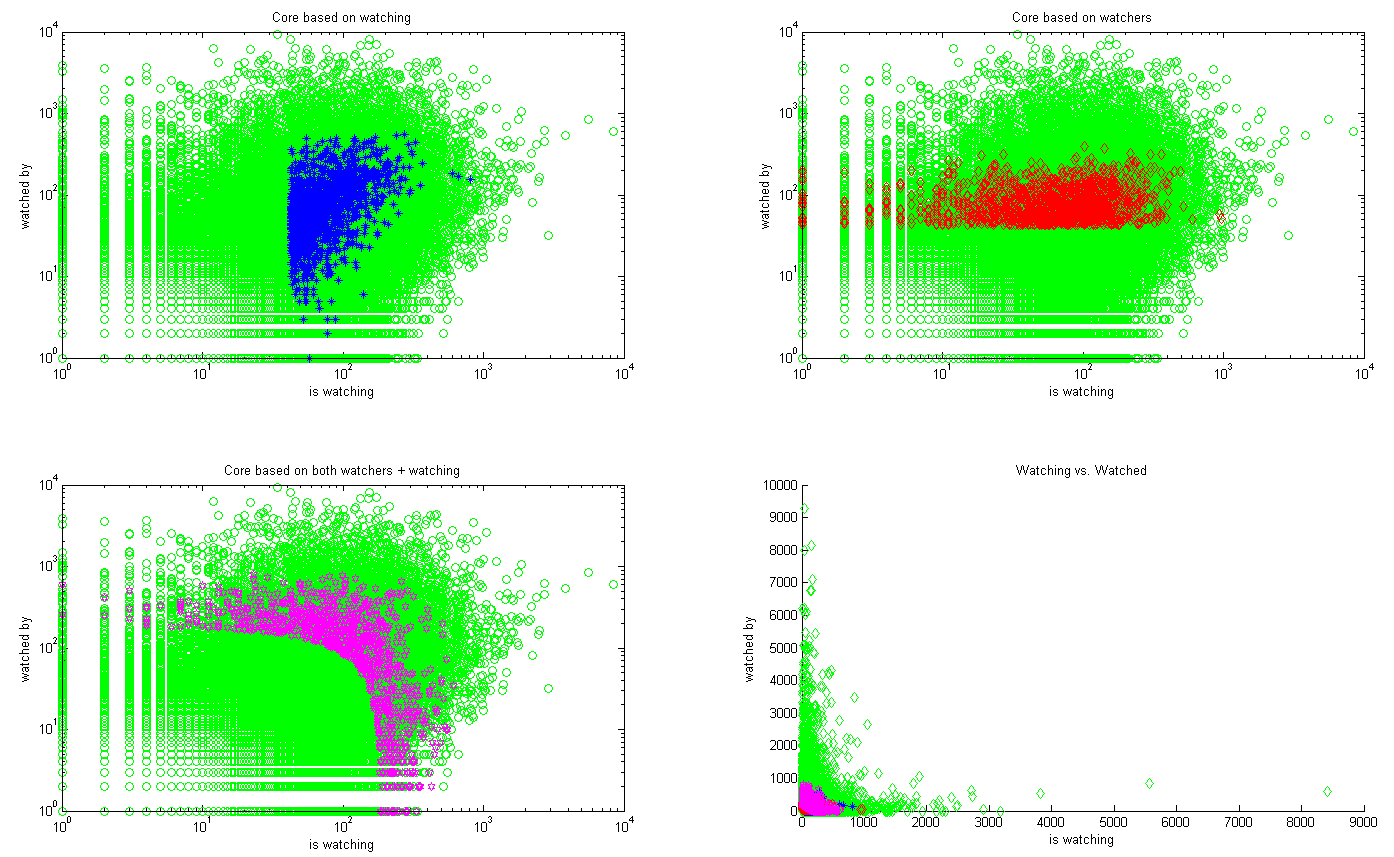
\includegraphics[width=1\linewidth]{img/core.png}
  \caption{Core network}
  \label{fig:results_core}
\end{figure}